\chapter{Floods and Droughts: Thailand}
\chapterauthor{Celine Liu, Heng Jia Min, Jeffrey Tong, Nathalie Baer Chan, and Sonia Kaur Sambhi}

\section{A Cycle of Floods and Droughts in Thailand}

From July to December 2010, as the rainy season reached its peak across Thailand, floodwaters from the north began inundating the central provinces, threatening to head south into Bangkok in what would turn out to be the worst flood disaster to hit Thailand in half a century (Gale \& Saunders, 2015). Just months before this incident, Thailand was still in the midst of battling its most serious drought in decades (Garbero, 2013). 

This cycle of floods and droughts, a common feature of life in Thailand, may seem puzzling given Thailand’s annual rainfall far exceeds its annual water demand, according to Sumet Tantivejkul, Utokapat Foundation chairman. During the Sustainable Water Management Forum 2016, Tantivejkul highlighted, ``[Thailand receives] around 754,000 million cubic metres of rain per year. That is more than enough for the annual water demand of around 100,000 million cubic metres\ldots However, only 5.7\% of rainfall, 70,370 million cubic metres, empties into the reservoirs.''

However, how floods and droughts arise are less to do with the volume of precipitation than the uneven distribution of precipitation across timescales and geographical locations, especially as it relates to the El Nino Southern Oscillation and the Indian Ocean Dipole. These distribution patterns interact with Thailand’s water resource management approaches such as dams and water use to, resulting in floods and droughts of varying severity.

\begin{figure}
	\centering
		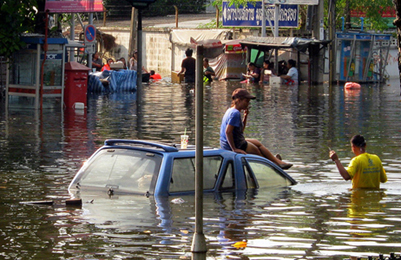
\includegraphics[width=0.50\textwidth]{Flood_Thailand.jpg}
	\caption{Figure 1: Floodwaters reach waist deep during the 2011 Thai Floods (Source: TBD).}
	\label{fig:Flood_Thailand}
\end{figure}


\section{Mechanisms of Floods and Droughts}

Floods are generated when a stream’s discharge exceeds the capacity of its channel, resulting in water inundating land that is normally dry. There are three main types of floods: coastal (surge) floods, pluvial (surface) floods and fluvial (river) floods. Coastal floods are caused by the inflow of saltwater (usually the result of a large storm or tsunami) from the ocean to inland areas, while pluvial and fluvial floods are caused by the runoff of water from the land, usually during excessive rain or sometimes ruptured dams (Maddox, 2014). 

Floods take hours or even days to develop. When there is rain, stream discharge gradually increases until it reaches a peak flow. Floods emerge when the stream discharge crosses a particular threshold (determined by the channel’s capacity), and can be categorised as flash floods when the time lag between intense rainfall and peak flow is very small (Figures 2 and 3; Skinner and Murck, 2011). Stream discharge is the product of the velocity, depth and width of water flowing through it. Channel capacity can be modelled by different equations, but Manning’s equation (1891) which applies to uniform flow in open channels is commonly used:

\begin{equation}
Q = VA = (\frac{1}{n})AR^{2/3}\sqrt{S}
\end{equation}
 
\noindent Where (in SI Units):

\begin{itemize}
	\item Q = Flow rate (m3/s)
	\item V = Velocity (m/s)
	\item A = Flow area (m2)
	\item n = Manning’s roughness coefficient (s/m1/3)the higher the coefficient, the greater the resistance to flow)
	\item R = Hydraulic radius (m)
	\item S = Channel slope (unitless)
\end{itemize}

Floods are classified based on their theoretical likelihood of occurring in a given time period. For example, a large destructive flood that is expected to happen only once every century is classified as a hundred-year-flood. What this theoretical likelihood translates to, in reality, is a one-percent chance that such a flood would happen in any given year. Unlike tectonic hazards, the occurrence of a flood of great magnitude does not reduce the probability of a flood of similar magnitude happening in the next year. Instead, after one flood season, the extensive ground saturation may make it even more difficult for water to infiltrate, increasing the likelihood of a flood in the next flood season (United States Geological Survey, 2018). 

\begin{figure}[htb]
	\centering
		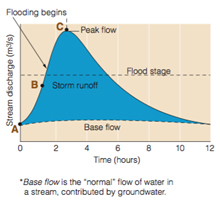
\includegraphics[width=1.00\textwidth]{graphics/base_flow.jpg}
	\caption{Hydrograph representation of the formation of floods (Source: Skinner and Murck, 2011).}
	\label{fig:base_flow}
\end{figure}
 
\begin{figure}[htbp]
	\centering
		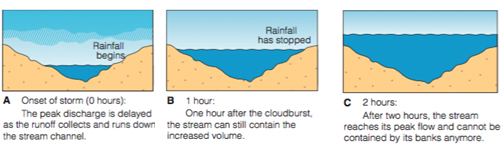
\includegraphics[width=1.00\textwidth]{graphics/hydrograph.jpg}
	\caption{Figure 3: Visual representation of flood formation in a waterway (Source: Skinner and Murck, 2011).}
	\label{fig:hydrograph}
\end{figure}
  

Drought as a physical phenomenon is difficult to define, as over 150 published definitions of drought in the 1980s (National Drought Mitigation Center (U.S.), 2018) might testify to. Wilhite and Glantz (1985) have classified the definitions into four approaches: meteorological, agricultural, hydrological, and socio-economic. Meteorological drought, which defines drought on the basis of a degree of dryness in comparison to an expected, normal amount, is what most researchers and articles refer to when discussing drought. Meanwhile, agricultural drought refers to drought as it relates to agriculture, such as its effects on plant water demand, soil water deficits, reduced groundwater, or topsoil moisture levels. Hydrological drought, which can lag behind meteorological and agricultural drought, concerns precipitation deficiencies in particular components of the hydrological system, such as groundwater and reservoir levels, streamflow and soil moisture. Socio-economic drought approaches then define drought with reference to demand and supply, such as Hoyt’s definition (1936) of drought as occurring “when precipitation is not sufficient to meet the needs of established human activities”. 

While we broadly refer to drought as a physical phenomenon arising from lower-than-average rainfall (meteorological drought) in this paper, we acknowledge that other definitions of drought contribute to the significance of drought to Thailand as well. For example, agricultural drought is important for Thailand where agriculture contributes 8-10% of its GDP every year (The World Bank, 2018), and where droughts can contribute to as much as 20 billion baht (634.3 million USD) losses in purchasing power among farmers, as in the case of the 2016 flood crisis (Thaiturapaisan, 2016). Hydrological drought is concerning given the 25 river basins and 254 sub-basins that Thailand possesses (The World Bank, 2011), which result in downstream effects that cannot be accounted for merely by local precipitation levels. Finally, socio-economic drought is concerning particularly for a country whose water demand is likely to continue increasing with urbanisation and economic development (The World Bank, 2011).

Interestingly, the probability of drought can increase following a flood, by disturbing the ability of water buffers to store the excess water as a water source during water-scarce periods. For example, during periods with normal levels of precipitation, water can infiltrate the ground as groundwater, but during a flood most of the precipitation enters the sea directly as runoff. Over time, the reduced groundwater supply can contribute to agricultural drought.

\section{Flood and Drought Meteorology}

\subsubsection{General Precipitation Trends}

Thailand is located between latitudes 6 and 20 degrees north. Its southern region experiences an equatorial climate with even rainfall throughout the year. Central and northern regions are characterized by a tropical monsoon climate with more clearly defined dry and wet seasons. 

\begin{figure}[htbp]
	\centering
		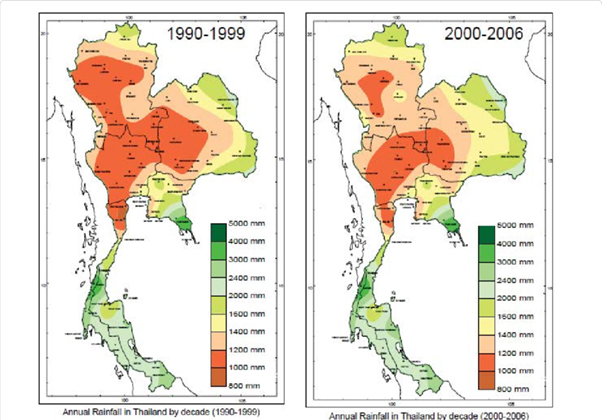
\includegraphics[width=1.00\textwidth]{graphics/Annual_Rainfall_Thailand.jpg}
	\caption{NOTE: Find better reference than this one.}
	\label{fig:Annual_Rainfall_Thailand}
\end{figure}

In particular, the climate of Thailand may be divided into three seasons as followed (Meteorological Department of Thailand):  

\begin{itemize}
	\item Rainy or southwest monsoon season (mid-May to mid-October). The southwest monsoon prevails over Thailand and abundant rain occurs over the entirety of the country, with 80\% of the average annual rainfall occurring during this period. During the wettest months of August and September rivers carry high runoffs and can overflow, leading to flooding (Figure 4). In extreme rainfall years the flooding may spread along Thailand's main water artery, the Chao Phraya River basin, towards Bangkok, the country's capital, before emptying into the sea.

\item Winter or northeast monsoon season (mid-October to mid-February). This is the mild period of the year in northern Thailand but the wettest point in the Southern East Coast, especially during October to November.  

\item Summer or pre-monsoon season (mid-February to mid-May). This is the transitional period from the northeast to southwest monsoons (Figure 4). The weather becomes warmer, especially in northern Thailand. Droughts are prevalent in the north during this period, while the south is generally protected due to its equatorial climate and more even rainfall.
\end{itemize}
